
%(BEGIN_QUESTION)
% Copyright 2006, Tony R. Kuphaldt, released under the Creative Commons Attribution License (v 1.0)
% This means you may do almost anything with this work of mine, so long as you give me proper credit

The following storage vessel holds water.  A pneumatic pressure transmitter located at the bottom infers water level by hydrostatic pressure (head).  Determine the calibration range of this pressure transmitter in order to properly translate the range of vessel level (0 to 18 feet) into an output signal of 3 to 15 PSI.  Please express the transmitter's calibration range in units of inches W.C. (inches of water column).

$$\includegraphics[width=15.5cm]{i00243x01.eps}$$

Then, determine the following (assuming the transmitter has been properly calibrated for the application):

\begin{itemize}
\item{} Transmitter output signal (PSI) at 12 feet of level
\item{} Water level at 5.9 PSI signal output
\end{itemize}

\underbar{file i00243}
%(END_QUESTION)





%(BEGIN_ANSWER)

Lower range-values (LRV): 0 inches W.C. input = 3 PSI output

\vskip 10pt

Upper range-values (URV): 216 inches W.C. input = 15 PSI output

\vskip 10pt

\begin{itemize}
\item{} Transmitter output signal (PSI) at 12 feet of level = 11 PSI
\item{} Water level at 5.9 PSI signal output = 4.35 feet
\end{itemize}

%(END_ANSWER)





%(BEGIN_NOTES)

%INDEX% Measurement, level: hydrostatic pressure

%(END_NOTES)


